\documentclass{beamer}
\usepackage[utf8]{inputenc}

\usetheme{Madrid}
\usecolortheme{default}
\usepackage{amsmath,amssymb,amsfonts,amsthm}
\usepackage{txfonts}
\usepackage{tkz-euclide}
\usepackage{listings}
\usepackage{adjustbox}
\usepackage{array}
\usepackage{tabularx}
\usepackage{gvv}
\usepackage{lmodern}
\usepackage{circuitikz}
\usepackage{tikz}
\usepackage{graphicx}

\setbeamertemplate{page number in head/foot}[totalframenumber]

\usepackage{tcolorbox}
\tcbuselibrary{minted,breakable,xparse,skins}



\definecolor{bg}{gray}{0.95}
\DeclareTCBListing{mintedbox}{O{}m!O{}}{%
  breakable=true,
  listing engine=minted,
  listing only,
  minted language=#2,
  minted style=default,
  minted options={%
    linenos,
    gobble=0,
    breaklines=true,
    breakafter=,,
    fontsize=\small,
    numbersep=8pt,
    #1},
  boxsep=0pt,
  left skip=0pt,
  right skip=0pt,
  left=25pt,
  right=0pt,
  top=3pt,
  bottom=3pt,
  arc=5pt,
  leftrule=0pt,
  rightrule=0pt,
  bottomrule=2pt,
  toprule=2pt,
  colback=bg,
  colframe=orange!70,
  enhanced,
  overlay={%
    \begin{tcbclipinterior}
    \fill[orange!20!white] (frame.south west) rectangle ([xshift=20pt]frame.north west);
    \end{tcbclipinterior}},
  #3,
}
\lstset{
    language=C,
    basicstyle=\ttfamily\small,
    keywordstyle=\color{blue},
    stringstyle=\color{orange},
    commentstyle=\color{green!60!black},
    numbers=left,
    numberstyle=\tiny\color{gray},
    breaklines=true,
    showstringspaces=false,
}
\begin{document}

\title 
{4.7.57}
\date{september 14,2025}


\author 
{Namaswi-EE25BTECH11060}
\frame{\titlepage}
\begin{frame}{Question}
Find distance of $\brak{3,-5}$ from line 3x-4y-26=0
\end{frame}
\begin{frame}{solution}
The given line is
\[
3x - 4y - 26 = 0
\]
This can be written in the form 
\begin{align}
\Vec{n}^\top \Vec{x} = c
\end{align}
where 
\[
\Vec{n}= \begin{pmatrix} 3 \\ -4 \end{pmatrix}, 
\quad c = 26.
\]

Let the point be 
\[
\Vec{P}= \begin{pmatrix} 3 \\ -5 \end{pmatrix}.
\]
\end{frame}
\begin{frame}{solution}
The distance of point \(P\) from the line is
\begin{align}
d = \frac{|\Vec{n}^\top \Vec{P} - c|}{\|\Vec{n}\|}.
\end{align}

\begin{align}
\Vec{n}^\top \Vec{P} = \begin{pmatrix} 3 & -4 \end{pmatrix}
\begin{pmatrix} 3 \\ -5 \end{pmatrix}\\
= 3(3) + (-4)(-5)\\ = 9 + 20 = 29.\\
\Vec{n}^\top \Vec{P} - c\\ = 29 - 26 = 3.\\
\|\Vec{n}\| = \sqrt{3^2 + (-4)^2}\\ = \sqrt{9+16} = 5.\\
So,
d = \frac{|3|}{5} = \frac{3}{5}.
\end{align}
\end{frame}
\begin{frame}[fragile]
    \frametitle{C Code}
    \begin{lstlisting}
#include <stdio.h>
#include <math.h>

int main() {
    // Line: 3x - 4y - 26 = 0
    double n[2] = {3, -4};   // normal vector
    double c = 26;
    double P[2] = {3, -5};   // point (3, -5)

    // Compute n^T * P
    double dot = n[0]*P[0] + n[1]*P[1];
\end{lstlisting}
\end{frame}
\begin{frame}[fragile]
    \frametitle{C Code }
    \begin{lstlisting}
 // Numerator |n^T P - c|
    double numerator = fabs(dot - c);
    // Denominator ||n||
    double norm = sqrt(n[0]*n[0] + n[1]*n[1]);
    // Distance
    double distance = numerator / norm;
    printf("Distance = %lf\n", distance);
    return 0;
}

\end{lstlisting}
\end{frame}
\begin{frame}[fragile]
\frametitle{Python Code}
\begin{lstlisting}
  import numpy as np
import matplotlib.pyplot as plt

# Line: 3x - 4y - 26 = 0
n = np.array([3, -4])   # normal vector
c = 26
P = np.array([3, -5])   # given point

# Foot of perpendicular formula: Q = P - ((n^T P - c)/||n||^2) * n
dot = n @ P
Q = P - ((dot - c) / (np.dot(n, n))) * n

# Prepare line for plotting
x_vals = np.linspace(-10, 10, 400)
y_vals = (3*x_vals - 26)/4   # from 3x - 4y - 26 = 0
\end{lstlisting}
\end{frame}


\begin{frame}[fragile]
\frametitle{Python Code}
\begin{lstlisting}

# Plot line
plt.plot(x_vals, y_vals, 'b', label=r'$3x-4y-26=0$')

# Plot point P
plt.scatter(P[0], P[1], color='red', zorder=5)
plt.text(P[0]+0.3, P[1]-0.3, 'P(3,-5)', fontsize=12, color='red')

# Plot foot of perpendicular Q
plt.scatter(Q[0], Q[1], color='green', zorder=5)
plt.text(Q[0]+0.3, Q[1]+0.3, f'Q({Q[0]:.2f},{Q[1]:.2f})', fontsize=12, color='green')

\end{lstlisting}
\end{frame}
\begin{frame}[fragile]
\frametitle{Python Code}
\begin{lstlisting}
# Dotted line PQ
plt.plot([P[0], Q[0]], [P[1], Q[1]], 'r--', label='Shortest Distance')

# Axes & labels
plt.axhline(0, color='black', linewidth=0.8)
plt.axvline(0, color='black', linewidth=0.8)
plt.gca().set_aspect('equal', adjustable='box')
plt.legend()
plt.grid(True, linestyle='--', alpha=0.6)
plt.title("Distance from Point to Line")
plt.show()
\end{lstlisting}
\end{frame}
\begin{frame}[fragile]
\frametitle{C and Python Code}
\begin{lstlisting}
import ctypes

# Load the shared object file
lib = ctypes.CDLL('./distance.so')

# Set argument and return types
lib.point_to_line_distance.argtypes = [ctypes.c_double, ctypes.c_double, ctypes.c_double,
                                       ctypes.c_double, ctypes.c_double]
lib.point_to_line_distance.restype = ctypes.c_double
\end{lstlisting}
\end{frame}
\begin{frame}[fragile]
\frametitle{C and Python Code}
\begin{lstlisting}
# Line: 3x - 4y - 26 = 0 → a=3, b=-4, c=-26
a, b, c = 3, -4, -26
px, py = 3, -5   # Point

# Call the C function
distance = lib.point_to_line_distance(a, b, c, px, py)
print(f"Distance from P({px},{py}) to line 3x-4y-26=0 is {distance}")
\end{lstlisting}
\end{frame}

\begin{frame}{Plot}
    \centering
    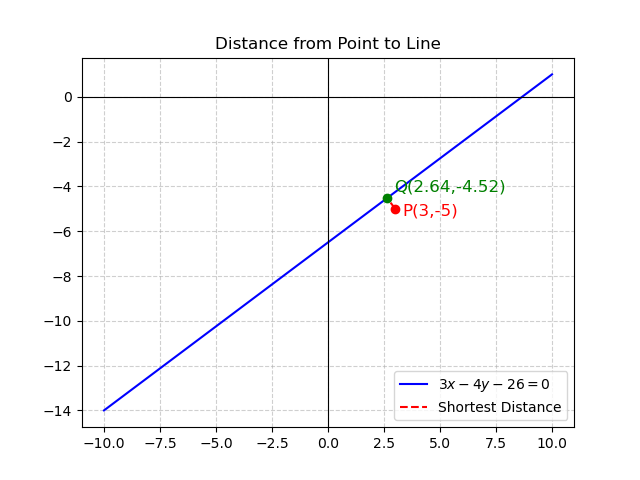
\includegraphics[width=\columnwidth, height=0.8\textheight, keepaspectratio]{Figure_7.png}     
\end{frame}
\end{document}